% --- LaTeX Presentation Template - S. Venkatraman ---

% --- Set document class ---

% Remove "handout" when presenting to include pauses
\documentclass[dvipsnames, handout]{beamer}
\usepackage{layout}
\usepackage{caption}
\usepackage{subcaption}
\usetheme{default}
\usepackage{textcomp}
\usepackage{pifont}
\usepackage{subcaption}
\usepackage{tabularx}
\usepackage[inline]{asymptote}


% Make content that is hidden by pauses "transparent"
\setbeamercovered{transparent}

% --- Slide layout settings ---

% Set line spacing
\renewcommand{\baselinestretch}{1.15}

% Set left and right text margins
\setbeamersize{text margin left=8mm, text margin right=8mm}


% Add slide numbers in bottom right corner
\setbeamertemplate{footline}[frame number]

% Remove navigation symbols
\setbeamertemplate{navigation symbols}{}

% Allow local line spacing changes
\usepackage{setspace}

% --- Color and font settings ---
% We will mainly use 2 colors: uofsc-red-primary, black
% We will use several font sizes to differentiate title, subtitle, normal text, etc.

\usepackage{xcolor}

% define theme colors
\definecolor{uofsc-red-primary}{HTML}{73000a}
\definecolor{uofsc-red-rose}{HTML}{cc2e40}
\definecolor{uofsc-red-dark}{HTML}{570008}

% Change itemized list bullets to circles
\setbeamertemplate{itemize item}{\color{uofsc-red-rose}$\bullet$}
\setbeamertemplate{itemize subitem}{\color{uofsc-red-rose}$\circ$}

\setbeamertemplate{enumerate item}{\color{uofsc-red-rose}\arabic{enumi}.}

% Slide title background color
\definecolor{background}{HTML}{ffffff}

% Slide title text color
\definecolor{titleText}{HTML}{73000a}

% Other possible color schemes

% - Light green/dark green -
%\definecolor{background}{HTML}{e4ede4}
%\definecolor{titleText}{HTML}{2e592f}

% - Light blue/dark blue -
%\definecolor{background}{HTML}{d5d9e8}
%\definecolor{titleText}{HTML}{2d375e}

% - Beige/dark blue -
%\definecolor{background}{HTML}{e8e2d5}
%\definecolor{titleText}{HTML}{2d3375}

% Set colors
\setbeamercolor{frametitle}{bg=background, fg=titleText}
\setbeamercolor{title}{fg=uofsc-red-primary}
\setbeamercolor{subtitle}{fg=uofsc-red-primary}

% Set font sizes for frame title and subtitle
\setbeamerfont{frametitle}{size=\fontsize{15}{16}}
\setbeamerfont{framesubtitle}{size=\small}

% --- Math/Statistics commands ---

% Add a reference number to a single line of a multi-line equation
% Usage: "\numberthis\label{labelNameHere}" in an align or gather environment
\newcommand\numberthis{\addtocounter{equation}{1}\tag{\theequation}}

% Shortcut for bold text in math mode, e.g. $\b{X}$
\let\b\mathbf

% Shortcut for bold Greek letters, e.g. $\bg{\beta}$
\let\bg\boldsymbol

% Shortcut for calligraphic script, e.g. %\mc{M}$
\let\mc\mathcal

% \mathscr{(letter here)} is sometimes used to denote vector spaces
\usepackage[mathscr]{euscript}

% Convergence: right arrow with optional text on top
% E.g. $\converge[p]$ for converges in probability
\newcommand{\converge}[1][]{\xrightarrow{#1}}

% Weak convergence: harpoon symbol with optional text on top
% E.g. $\wconverge[n\to\infty]$
\newcommand{\wconverge}[1][]{\stackrel{#1}{\rightharpoonup}}

% Equality: equals sign with optional text on top
% E.g. $X \equals[d] Y$ for equality in distribution
\newcommand{\equals}[1][]{\stackrel{\smash{#1}}{=}}

% Normal distribution: arguments are the mean and variance
% E.g. $\normal{\mu}{\sigma}$
\newcommand{\normal}[2]{\mathcal{N}\left(#1,#2\right)}

% Uniform distribution: arguments are the left and right endpoints
% E.g. $\unif{0}{1}$
\newcommand{\unif}[2]{\text{Uniform}(#1,#2)}

% Independent and identically distributed random variables
% E.g. $ X_1,...,X_n \iid \normal{0}{1}$
\newcommand{\iid}{\stackrel{\smash{\text{iid}}}{\sim}}

% Sequences (this shortcut is mostly to reduce finger strain for small hands)
% E.g. to write $\{A_n\}_{n\geq 1}$, do $\bk{A_n}{n\geq 1}$
\newcommand{\bk}[2]{\{#1\}_{#2}}

% Math mode symbols for common sets and spaces. Example usage: $\R$
\newcommand{\R}{\mathbb{R}}	% Real numbers
\newcommand{\C}{\mathbb{C}}	% Complex numbers
\newcommand{\Q}{\mathbb{Q}}	% Rational numbers
\newcommand{\Z}{\mathbb{Z}}	% Integers
\newcommand{\N}{\mathbb{N}}	% Natural numbers
\newcommand{\F}{\mathcal{F}}	% Calligraphic F for a sigma algebra
\newcommand{\El}{\mathcal{L}}	% Calligraphic L, e.g. for L^p spaces

% Math mode symbols for probability
\newcommand{\pr}{\mathbb{P}}	% Probability measure
\newcommand{\E}{\mathbb{E}}	% Expectation, e.g. $\E(X)$
\newcommand{\var}{\text{Var}}	% Variance, e.g. $\var(X)$
\newcommand{\cov}{\text{Cov}}	% Covariance, e.g. $\cov(X,Y)$
\newcommand{\corr}{\text{Corr}}	% Correlation, e.g. $\corr(X,Y)$
\newcommand{\B}{\mathcal{B}}	% Borel sigma-algebra

% Other miscellaneous symbols
\newcommand{\tth}{\text{th}}	% Non-italicized 'th', e.g. $n^\tth$
\newcommand{\Oh}{\mathcal{O}}	% Big-O notation, e.g. $\O(n)$
\newcommand{\1}{\mathds{1}}	% Indicator function, e.g. $\1_A$

% Additional commands for math mode
\DeclareMathOperator*{\argmax}{argmax}	% Argmax, e.g. $\argmax_{x\in[0,1]} f(x)$
\DeclareMathOperator*{\argmin}{argmin}	% Argmin, e.g. $\argmin_{x\in[0,1]} f(x)$
\DeclareMathOperator*{\spann}{Span}	% Span, e.g. $\spann\{X_1,...,X_n\}$
\DeclareMathOperator*{\bias}{Bias}	% Bias, e.g. $\bias(\hat\theta)$
\DeclareMathOperator*{\ran}{ran}		% Range of an operator, e.g. $\ran(T) 
\DeclareMathOperator*{\dv}{d\!}		% Non-italicized 'with respect to', e.g. $\int f(x) \dv x$
\DeclareMathOperator*{\diag}{diag}	% Diagonal of a matrix, e.g. $\diag(M)$
\DeclareMathOperator*{\trace}{trace}	% Trace of a matrix, e.g. $\trace(M)$
\DeclareMathOperator*{\supp}{supp}	% Support of a function, e.g., $\supp(f)$

% --- Presentation begins here ---

\begin{document}

% --- Title slide ---
% We have to specify the location of title, subtitle, author, dates, institutes, etc
% Right now we just put everything on the slides, without specifying the space between rows or the height of blocks.
% We will fix these details later.
% In general, we don't want to have too many different font sizes to mess up a page. The names, dates, affiliations (institutes, emails) should be of the same font size, except for some extreme cases (for example, the affiliation is too long and it has to be shrank to be fitted into the page).
% The space between title (including subtitle) to author to affiliation should keep constant. It's not the absolute location but the space in between that determines the overall look of the page.
% We will design this better, with reference to https://www.overleaf.com/learn/latex/Beamer


\title{3D Finger Motion Tracking Using Ultrasound and Millimeter-Wave Sensing}
\subtitle{Project Proposal}
\author{Zifei (David) Zhong, Guangyi (Simona) Chen\vspace{-.3cm}}

\institute{Dept. of Computer Science and Engineering,\\University of South Carolina}
\date{}
\begin{frame}
\titlepage
\vspace{-1.2cm}
\begin{center}

\includegraphics[width=1cm]{imgs/uofsc-logo.png}\bigskip
%{\begin{spacing}{1.2}\scriptsize 
%Joint work with FirstName LastName, FirstName LastName
%\end{spacing}}
\end{center}
\end{frame}

% --- Main content ---

% Example slide: use \pause to sequentially unveil content
\begin{frame}[t]{Introduction}
%\framesubtitle{Collecting data from consumer wearables}

\begin{itemize}
\item 3D finger motion tracking has a wide range of applications
\begin{enumerate}
\item Virtual Reality
\item Gaming
\item Sign Language Recognition
\item other
\end{enumerate}

\item Limitations of Existing Solutions
\begin{enumerate}
\item Camera-based solutions: privacy concerns, light condition
\item Hand Gesture Classification: specific to applications
\end{enumerate}
\end{itemize}
\end{frame}


\begin{frame}[t]{Related Work}
%\framesubtitle{Collecting data from consumer wearables}

\begin{itemize}
\item Ultrasound imaging 
\begin{enumerate}
\item SoundSense: 12 gestures, 82.2\% accuracy, 2012
\item Feng \& Lai: 4 gestures, 99.8\% accuracy, 2021
\item EchoFlex: 10 gestures, 98\% accuracy, 2017
\item FingerIO: gesture classification, 2016
\end{enumerate}

\item mmWave imaging
\begin{enumerate}
\item mm4arm: 3D finger motion tracking, 2023
\item mmASL: asl classification, 87\% accuracy, 2020
\item ExASL: asl classification, 83.5\% accuracy, 2020
\item DeafSpaces: asl classification, 15 gestures, 2021
\item Google Soli: 9 gestures, 2016
\end{enumerate}

\end{itemize}
\end{frame}

\begin{frame}[t]{Project Proposal}
%\framesubtitle{Collecting data from consumer wearables}

\begin{itemize}
\item Fine-grain 3D Finger Motion Tracking 
\begin{enumerate}
\item Ultrasound: less lossy data
\item Millimeter-Wave: better resolution
\item Fusion of ultrasound and millimeter-wave reflections
\end{enumerate}

\item Advantages
\begin{enumerate}
\item privacy-preserved
\item applied to wider range of environments, including dark environment
\item advantages from both ultrasound and mmWave techniques
\item better accuracy in tracking 3D finger motions
\end{enumerate}

\end{itemize}
\end{frame}

\begin{frame}[t]{An Example}
\begin{itemize}
\item Instead of classifying a set of discrete hand gestures, we intend to reconstruct 3D finger motion at the joint-level.
\end{itemize}
\begin{center}
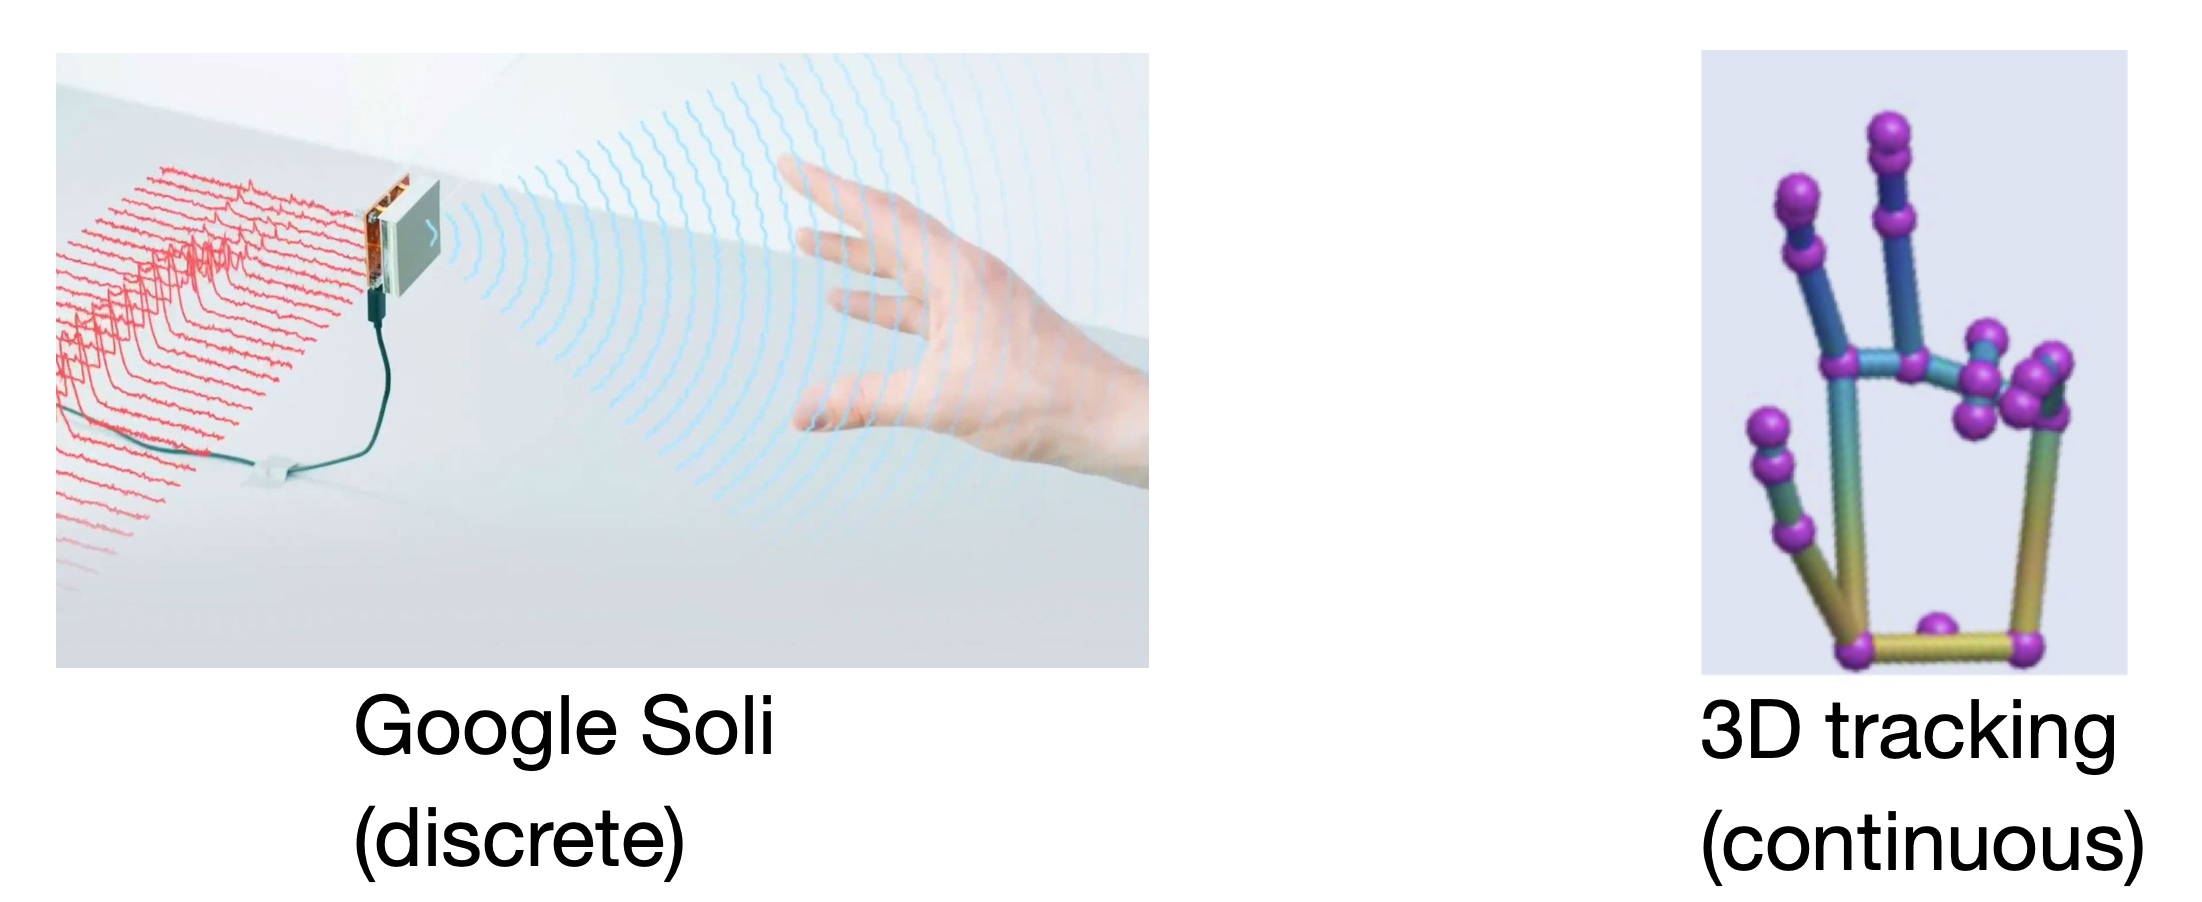
\includegraphics[width=0.8\textwidth]{imgs/example-3d-finger-motion.jpg}
\end{center}
\end{frame}

\begin{frame}[t]{Hardware}
\begin{itemize}
\item Ultrasound device
\begin{enumerate}
\item MAXQ7667
\item Frequency: 13m Hz - 16m HZ
\end{enumerate}
\item Millimeter-Wave device
\begin{enumerate}
\item IWR1443BOOST
\item 3 TX, 4 RX
\item Frequency: 76G Hz - 86G Hz
\end{enumerate}
\end{itemize}


\begin{figure}[ht]
\begin{subfigure}[b]{0.4\textwidth}
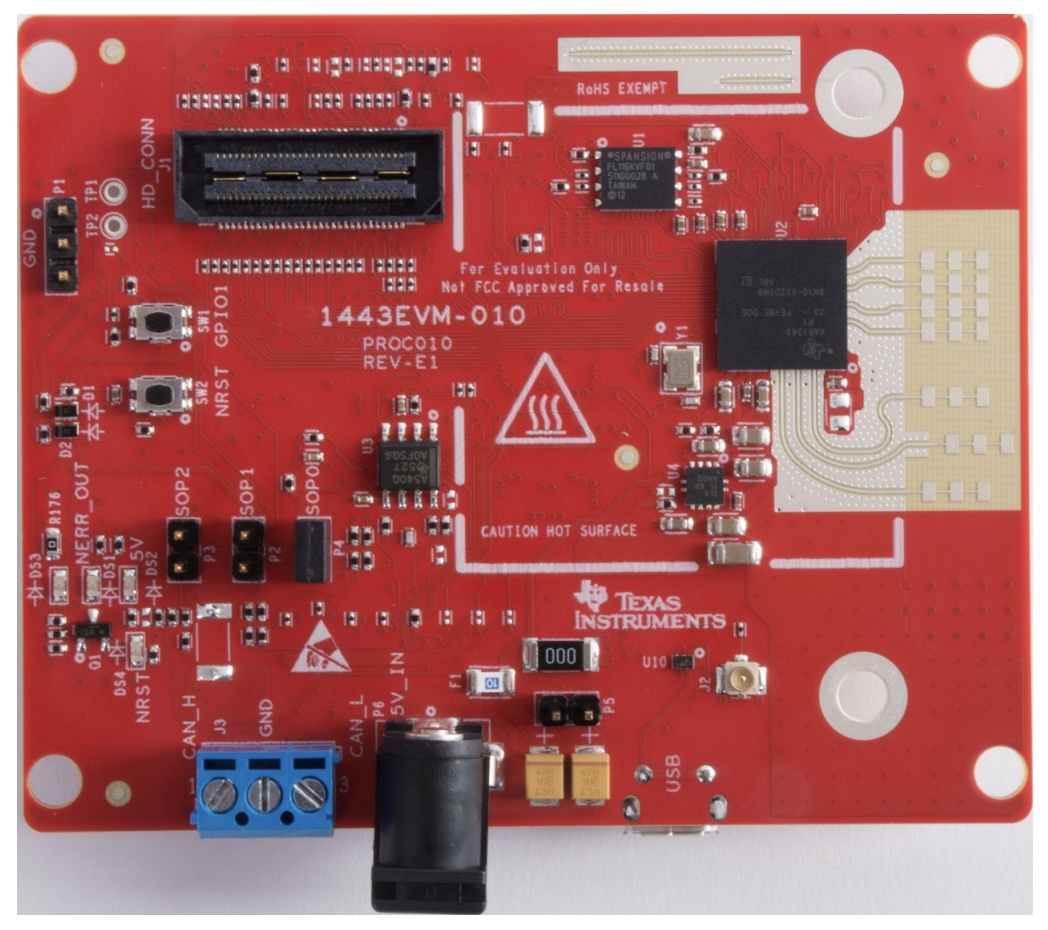
\includegraphics[width=\textwidth]{imgs/iwr1443boost.jpg}
\end{subfigure}
\begin{subfigure}[b]{0.4\textwidth}
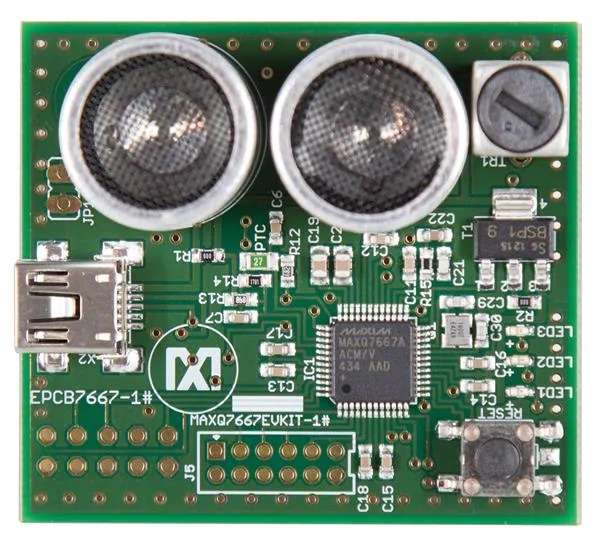
\includegraphics[width=\textwidth]{imgs/maxq7667evkit.jpg}
\end{subfigure}
\end{figure}


\end{frame}

\begin{frame}[t]{Challenges}
\begin{itemize}
\item It's the first work that combines ultrasound and millimeter-wave imaging techniques to track 3D finger motions.
\item Ground truth database?
\item High resolution sensors in lightning environment
\end{itemize}
\end{frame}

\begin{frame}[t]{Timelines}

\begin{center}
\begin{tabular}{|c|c|}
\hline
work  & finish date \\
\hline
\hline
{\tiny Data collection} & {\tiny March 7}\\
\hline
 {\tiny Fusion algorithm and testing } & {\tiny April 20}\\
\hline 
{\tiny Finalizing} & {\tiny April 27} \\
\hline
\end{tabular}
\end{center}

\end{frame}

% --- Bibliography slide ---

%\begin{frame}{References}
%\begin{thebibliography}{10}
%\beamertemplatearticlebibitems
%{\small

%\bibitem{Paper1}
%Paper 1 Title.
%\newblock Paper 1 Authors. \\
%{\it Journal Name} Edition, Year.

%\bibitem{Paper 2}
%Paper 2 Title.
%\newblock Paper 2 Authors.\\
%arXiv:1234.56789.
%}
%\end{thebibliography}
%\end{frame}

% --- Thank you slide ---

%\begin{frame}
%\begin{center}
%{\large\color{titleText} Thank you!}
%\vspace{1cm}

%Zifei (David) Zhong \\[1em]
%zhongz@email.sc.edu \\
%https://zfz.github.io
%\end{center}
%\end{frame}

% --- Presentation ends here ---

\end{document}
